\documentclass{IEEEtran}
\usepackage[spanish]{babel}
\usepackage[utf8]{inputenc}
\usepackage{authblk}
\usepackage{amsmath}
\usepackage{subfig}
\usepackage{graphicx}
\usepackage{cite}

\title{Evaluación de Estrategias de Obtención de Mediciones EIT para Rastreo de Dispersión de líquidos. }
\author[1]{O. F. Cándido-Sánchez}
\author[1]{J. A. Gutiérrez-Gnecchi}
\affil[1]{Departamento de Ingeniería Electrónica, Instituto Tecnológico de Morelia}

\begin{document}
  \maketitle
    %Abstract
  \begin{abstract}
  \end{abstract}

  %Keywords
  \begin{IEEEkeywords}
  \end{IEEEkeywords}

  \section{Introducción}
En la última década, la tomografía de impedancia eléctrica (Electrical Impedance Tomography: \textit{EIT}) ha recibido considerable atención por parte de la comunidad científica en el mundo para aplicaciones médicas e industriales. En medicina, EIT es una herramienta que puede ser aplicable para rastrear la difusion de medicamentos quimioterapeúticos para tratamiento de cáncer de mama\cite{Gnecchi2018}.\\
El estudio de cancer de mama por EIT está aprobado por la FDA para ayudar a clasificar los tumores encontrados en los mamogramas. Sin embargo, hasta el momento no se han realizado suficientes pruebas clínicas para que se pueda usar en pruebas de detección del cáncer de seno \cite{Cancer.org}. La EIT podría usarse como complemento de la mamografía y la ecografía para la detección del cáncer de mama. Sin embargo, la diferenciación de las lesiones malignas de las benignas en función de las mediciones de impedancia requiere más investigación\cite{Zou2003}.\\
En general, el objetivo de la \textit{EIT} es el de reconstruir imágenes, las cuales representan una sección transversal de una distribucion espacial de impedancia eléctrica interna de un objeto, ya sea en dos o tres dimensiones \cite{Mendoza2012}.\\
Este trabajo está dedicado a proponer una metodología para obtener, reconstruir y analizar mediciones EIT que permitan proponer modelos matemáticos de procesos que involucren la dispersión de líquidos en medios permeables.\\
\section{Estado del arte}
La tomografía de impedancia eléctrica (EIT) es una técnica de imagen para estimar la distribución de la conductividad eléctrica de un objeto. En aplicaciones industriales, EIT se ha aplicado para detectar la distribución de aire, burbujas de aire y grietas en tuberías. En las aplicaciones geofísicas, EIT puede aplicarse para proporcionar información de estimación de saturación de un depósito y la medida de contenido de mineral en la tierra.
En las aplicaciones médicas, EIT se ha aplicado para controlar el vaciado gástrico, controlar la función pulmonar, la función cardíaca, la función nerviosa, la cantidad de agua en los pulmones y detectar el cáncer de mama apartir de la detección y la caracterización de los tumores\cite{Wang2011}.

EIT fue introducido a principios de la década de 1980 por Barber y Brown. Al poco tiempo después, se sugirió un amplio espectro de posibles aplicaciones en medicina, que van desde el vaciado gástrico hasta el monitoreo de la función cerebral y desde la imagenología de los senos a la evaluación de la función pulmonar\cite{Teschner2015}.

El principio básico de medición de la biompedancia para el diagnóstico considera que diferentes materiales tienen diferentes propiedades eléctricas. Un procedimiento común utiliza una combinación de componentes de conductividad y permitividad para representar las propiedades eléctricas de los tejidos. A bajas frecuencias, puede haber un efecto predominantemente resistivo, mientras que el efecto capacitivo aumenta a medida que aumenta la frecuencia de la señal de excitación.
Las variaciones de los componentes resistivos y capacitivos en función de la frecuencia se denominan dispersiones \cite{Schwan2003}.
\section{Objetivos}
\subsection{Objetivo general}
Reconstruir imágenes a partir de mediciones EIT en tejido ex-vivo para  rastreo de dispersion de liquidos.

\section{Metodología}
La tomografía de impedancia eléctrica se basa en una número de electrodos unidos a la periferia del objeto para ser estudiado,a diferencia de la tomografía de rayos X, donde las placas de excitación y detección pueden girar alrededor del objeto. En EIT los electrodos se fijan equidistantemente alrededor del objeto, en general, una señal de voltaje es generada, la señal de voltaje se convierte en corriente a través de un VCCS (fuente de corriente controlada por voltaje) y pasa a través de un multiplexor como se muestra en la figura 1. El multiplexor sera el encargado de seleccionr qué pares de electrodos se utilizaran para el flujo de corriente \cite{Gnecchi2010}.
\begin{figure}[h!]
\centering
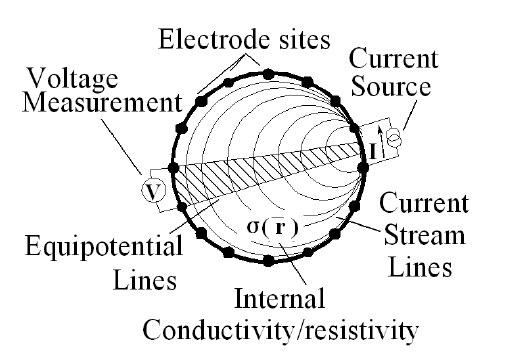
\includegraphics[width=2.5in]{imagen1}
\caption{Principio de medicion por EIT}\label{ref:FiguraA}
\end{figure}

\bibliographystyle{IEEEtran}
\bibliography{bibliography}

\end{document}
